\documentclass{sigkddExp}
\usepackage{amsmath}
\usepackage{graphicx}
\usepackage{titlesec}
\usepackage{hyperref}
\begin{document}

%
% --- Author Metadata here ---
% -- Can be completely blank or contain 'commented' information like this...
%\conferenceinfo{WOODSTOCK}{'97 El Paso, Texas USA} % If you happen to know the conference location etc.
%\CopyrightYear{2001} % Allows a non-default  copyright year  to be 'entered' - IF NEED BE.
%\crdata{0-12345-67-8/90/01}  % Allows non-default copyright data to be 'entered' - IF NEED BE.
% --- End of author Metadata ---

\title{Mortality Prediction of ICU Diabetic Patients, Based on Clinical History and Clinical Notes - A Multi-Network Deep Learning Model}
%\subtitle{[Extended Abstract]
% You need the command \numberofauthors to handle the "boxing"
% and alignment of the authors under the title, and to add
% a section for authors number 4 through n.
%
% Up to the first three authors are aligned under the title;
% use the \alignauthor commands below to handle those names
% and affiliations. Add names, affiliations, addresses for
% additional authors as the argument to \additionalauthors;
% these will be set for you without further effort on your
% part as the last section in the body of your article BEFORE
% References or any Appendices.

\numberofauthors{3}
%
% You can go ahead and credit authors number 4+ here;
% their names will appear in a section called
% "Additional Authors" just before the Appendices
% (if there are any) or Bibliography (if there
% aren't)

% Put no more than the first THREE authors in the \author command
%%You are free to format the authors in alternate ways if you have more 
%%than three authors.

\author{
%
% The command \alignauthor (no curly braces needed) should
% precede each author name, affiliation/snail-mail address and
% e-mail address. Additionally, tag each line of
% affiliation/address with \affaddr, and tag the
%% e-mail address with \email.
\alignauthor Olabisi Balogun\\
       \email{olb2@illinois.edu}
\alignauthor Jorge Flores\\
       \email{jorgedf2@illinois.edu}
\alignauthor Francisco Noya\\
       \email{fnoya2@illinois.edu}
}
\date{09 May 2021}
\maketitle
\begin{abstract}
       Diabetes is a very serious condition that can lead to serious consequences 
       and increase the risk of death when a patient is admitted in the ICU. In this paper,
 we explore the possibility of using clinical notes as well as lab and chart events 
 in a multi-network model where we process the clinical notes in a time series 
 RNN with dual-attention network, and the lab and chart events in another RNN,
 also with multi-attention, then merge them into a single multi-network model 
 to try to predict mortality of diabetic patients. Our combined model achieved 
 an AUC ROC score of 0.977 while this score fell to 0.905 or to 0.883, respectively,
 when either the clinical notes or the events data were ignored.  Furthermore,
 we were able to identify glucose level, patient weight, blood pressure,
 temperature, heart rate and oxygen saturation as the most relevant 
 factors for predicting the risk of death in this cohort.
\end{abstract}

\textbf {Abbreviations:} CNN – Convolutional Neural Network, 
UMLS – Unified Medical Language System, 
ICU – Intensive Care Unit, 
RNN - Recurrent Neural Networks, 
ICD - International Classification of Disease,
GRU – Gated Recurrent Unit.

\section{Introduction}
Diabetes mellitus comprises various medical conditions that are associated with hyperglycemia and it can 
be caused by an abnormal secretion of insulin in the body system (\cite{egan}). 
The number of diabetic patients worldwide has soared in the last 20 years (\cite{zimmet}). 
This increment has led to various studies on the efficient management of this condition. 
Diabetes has contributed to a 75\% increase in mortality rate:
a diabetic adult is at higher risk of death from other diseases compared to a 
non-diabetic adult in the US (\cite{gregg}). Therefore,
an efficient and timely interventional clinical decision support system that 
would aid in preventing death or predicting mortality would 
lead to a major milestone in diabetes management research. Anand et al., (\cite{anand}) stated 
that having diabetes could affect the treatment 
of ICU patients as unique factors have to be taken into consideration, for example,
glucose levels. Diabetic patients account for more than 45\% of ICU stays and consume 
more resources compared to patients suffering from 
other chronic diseases (\cite{anand}). 
 
Our research study aims to build a multi-network deep learning model to predict the mortality 
of ICU diabetic patients using the clinical notes,
and features from the Apache II scoring system plus features such as glycosylated hemoglobin (HbA1c),
serum creatinine, and glucose levels, that can improve the predictability for diabetic patients (\cite{anand}).

\section{Previous Work}
Research in diabetes is broad and different studies have engaged machine learning algorithms to improve 
the treatment and management of this global metabolic disorder. We streamlined past works to those that 
interest us most, which were done in the past five years and targeted a prediction task.
Anand et al., (\cite{anand}) employed binomial logistic regression to predict the risk mortality of ICU diabetic patients.  
Their research was based on the certainty that these variables (HbA1c, mean glucose during stay, serum creatine, 
diagnoses upon admission, and type of admission) were the major features needed for mortality prediction. 
Their research used the data from the MIMIC-III database and their model achieved ROC AUC value of 0.787.

Ye, Yao, Shen, Janarthanam \& Luo (\cite{ye}) employed different machine learning algorithms and knowledge-guided 
feature extraction to predict mortality in critically ill diabetic patients. Knowledge-guided CNN using CUI 
(UMLS concept unique identifiers) plus word embedding and CNN using word embedding were applied to clinical notes 
to predict mortality in diabetic ICU patients. They also ran different machine learning models such as Logistic Regression,
 Random Forest, XGBoost, Gradient Boosting, Deep Learning ANN, and Majority Voting with Majority Voting model taking 
 the lead with an AUC of 0.87. These machine learning algorithms were used with structured EHR data to predict mortality 
 risk in ICU diabetic patients. CNN with word embedding performed best overall with ROC AUC of 0.97.

Yang, Kuang \& Xia (\cite{yang}) proposed a multimodal deep learning neural network,
 which uses time series data and clinical notes to predict mortality of ICU patients,
 and obtained an ROC AUC of 0.861. Che, Purushotham, Cho, Sontag, \& Liu (\cite{che}) built a 
 model \textsc{GRU\_D} based on Gated Recurrent Unit (GRU),
 which could handle missing data, for mortality prediction using the time series features including input events,
 output events, lab events, and prescription events from the \textit {MIMIC III} dataset.
Choi, Bahadori, Kulas, Schuetz, Stewart and Sun (\cite{choi}) explored the use of multi RNNs with multi attention at different
 levels of granularity. We are going to apply a similar mechanism on each of the different networks,
 notes and events.

\section {Approach and implementation}
\subsection{Problem formulation}
The EHR information of a patient that is admitted into ICU can be represented 
as a timeseries of multiclass, multivariate observations, in our case, we will
 pay attention to two classes, chart/lab events and clinical notes. Considering $\mathit{v_i}$ a multi-hot vector 
 of the values for the different types of events observed in the date $\mathit{i}$, and $\mathit {n_i}$ an aggregate 
 notes embedding for all the notes registered in the date $\mathit{i}$. Being $\mathit {T_p}$ the number of dates with either events or notes registered 
 for the patient $\mathit {p}$. 
 At each date $\mathit{i}$, we can represent the patient $\mathit{p}$ with the tuple $\mathit {[v_i^{(p)}, n_i^{(p)}]}$ where $\mathit {i = 1 \ldots T_p}$. 
   
  The goal of our network is to predict the labels $\mathit {y(p) \in \{0,1\}}$ where 0 means the patient is predicted to be alive 48 hrs 
  after $\mathit {T_p}$, and 1 is predicted to be deceased.

  \subsection{Data Source}
  For our project, we  used the data from MIMIC-III database, because this is a very complete
  source with a lot of good real-life records of patients who have been admitted to ICU. 

\subsection{Cohort Selection}
First, we defined our cohort as patients who have a diabetic diagnosis, that is,
ICD-9 codes containing the word ``diabetes'' exempting codes 3572, V771, V180, V1221. 
We considered all the data of each patient from the moment they were first admitted, 
all the way to 48 hrs before last discharge. Some patients had multiple admissions, so 
we chose the observation window to be the earliest admission time to 48 hrs before the 
last discharge time. Any patient who did not have any data 48 hrs before final 
discharge was removed from the analysis. We used the presence of ``deathtime'' in the 
Admissions table to create a mortality flag: zero for alive and one for dead. 
The summary statistics of the cohort is depicted in the Table \ref{tab:cohort-stats}.

\begin{table}[h]
       \centering
       \caption{Cohort statistics}
       \label{tab:cohort-stats}
       \begin{tabular}{|c|c|} \hline
       Number of Cohort Patients&9822\\ \hline
       Maximum Length of Stay & 116 days\\ \hline
       Minimum Length of Stay& $\mathtt{<}$1 day\\ \hline
       \end{tabular}

\end{table}

The statistics of the Clinical Notes are shown in Table \ref{tab:notes-stats}.

\begin{table}
       \centering
       \caption{Clinical notes statistics}
       \label{tab:notes-stats}
       \begin{tabular}{|c|c|} \hline
       Min \# of notes per patient &0\\ \hline
       Max \# of notes per patient & 505 \\ \hline
       Avg. \# of notes per patient & 13\\ \hline
       \end{tabular}
\end{table}

The statistics of the Clinical / Lab events we used for the Events Network are shown in Table \ref{tab:events-stats}.

\begin{table*}
       \centering
       \caption{Statistics of selected features from chart events and lab events.}
       \label{tab:events-stats}
       \begin{tabular}{|l|c|c|c|c|c|} \hline
        & \multicolumn {5}{|c|}{Characteristics} \\ \hline
       &Count&Avg&Std Dev&Min&Max \\ \hline       
       \multicolumn{6}{|l|}{\textbf{APACHE II Features}} \\ \hline
       Diastolic blood pressure&7038135&56&220&-40&114108\\ \hline
       Fraction inspired oxygen&3489&1.26&0.91&0&10\\ \hline
       Glascow coma scale eye opening&1521073&3.28&1.06&1&4\\ \hline
       Glascow coma scale motor response&565486&5.29&1.39&1&6\\ \hline
       Glascow coma scale total&945427&11.43&3.74&3&15\\ \hline
       Glascow coma scale verbal response&565912&3.09&1.89&1&5\\ \hline
       Glucose&1570663&140&1143&-124&999999\\ \hline
       Heart Rate&7941588&102&3548&-88&9999999\\ \hline
       Height&12015&168.75&15.23&0&445\\ \hline
       Mean blood pressure&6363937&78&100&-135&120130\\ \hline
       Oxygen saturation&173361&88&22&0.8&6363\\ \hline
       Respiratory rate&7439791&19&863&-1&2355555\\ \hline
       Systolic blood pressure&6386370&119&125&-69&141146\\ \hline
       Temperature&129290&37&1&0&43\\ \hline
       Weight&1628937&84.63&24.61&0&300\\ \hline
       pH&530657&7.38&0.09&0&7.99\\ \hline
       \multicolumn{6}{|l|}{\textbf{Diabetes related Features}}\\ \hline
       HbA1C&16619&6.76&1.66&0.45&22\\ \hline
       Blood Glucose&749156&131&66&0&3565\\ \hline
       Serum Creatinine&797231&1.56&1.89&0&808\\ \hline
       \end{tabular}
\end{table*}

\subsection {Data Processing}
The \textit{MIMIC-III} database is available for access via \textsc{AWS} without need to download. 
We created a cohort master table (\textsf{diabetes\_patient\_cohort}), which we later used to 
create the source of information for each of our networks, notes and events. Using 
SQL queries, we created tables such as:
\begin{itemize}
       \item \textsf{diabetic\_patients\_notes\_agg} contains the notes of a patient aggregated by distinct 
date by concatenating the notes for that date if there are more than one.
      \item \textsf{diabetic\_patients\_events} contains the actual values for the different laboratory tests, 
vital signs and other values from ICU charts that we selected as features.  The data is 
aggregated by patient and date.  If multiple readings were obtained for the same feature 
of a patient on the same date, the daily average of it was used.
\end{itemize}

We split the \textsf{diabetic\_patient\_cohort} into train and evaluation sets using a split ratio of 
80\% to 20\%.  We called this our ``unbalanced'' cohort. We observed that the data has an inherent 
class imbalance. To resolve this issue, we oversampled the minority class in the training 
set to create a ``balanced'' cohort. All these actions were done using the \textsf{sklearn} library, 
\textsf{class resample} and stored on \textsc{S3 bucket} to later load onto \textsc{AWS Athena} tables: (\textsf{train\_cohort} 
and \textsf{test\_cohort}).

\subsection{Clinical Notes Embeddings}
We formed a notes table for the diabetic patients in the ICU by aggregating the notes for a given date. 
Then, we preprocessed the notes and trained our own word embedding model using the \textsf{Word2Vec} class from 
the \textsf{gensim.models} package. Once we had our embedding model, we processed each \textit{i-th} distinct date aggregated 
notes for every patient \textit{p} to obtain $\mathit n_i^{(p)}$ by calculating an embedding vector for each day 
notes.  We achieved this by obtaining the embedding vector for each word and then by adding the embeddings for all the 
words of the notes of the date \textit{i}. 

Figure \ref{fig:tSNE} shows a representation of the notes embedding using tSNE.

\graphicspath{ {figures/} } 
\begin{figure}\centering
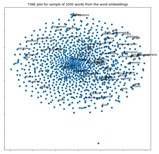
\includegraphics[width=1\columnwidth]{tSNE.png}
\caption{Word embeddings projected into 2D by means of tSNE.}
\label{fig:tSNE}
\end{figure}

\subsection{Events Embeddings}\clubpenalty10000000
The lab and clinical events corresponding to the selected features (see Table \ref{tab:events-stats})
had continuous numerical values. Therefore, the values registered in date \textit{i}
were averaged by feature. $\mathit v_i^{(p)}$ was constructed as a multi-hot vector in which
the index corresponds to the feature code and the value to the average of each feature for date \textit{i}.

\subsection{Neural Network Model}

\graphicspath{ {figures/} } 
\begin{figure*}\centering
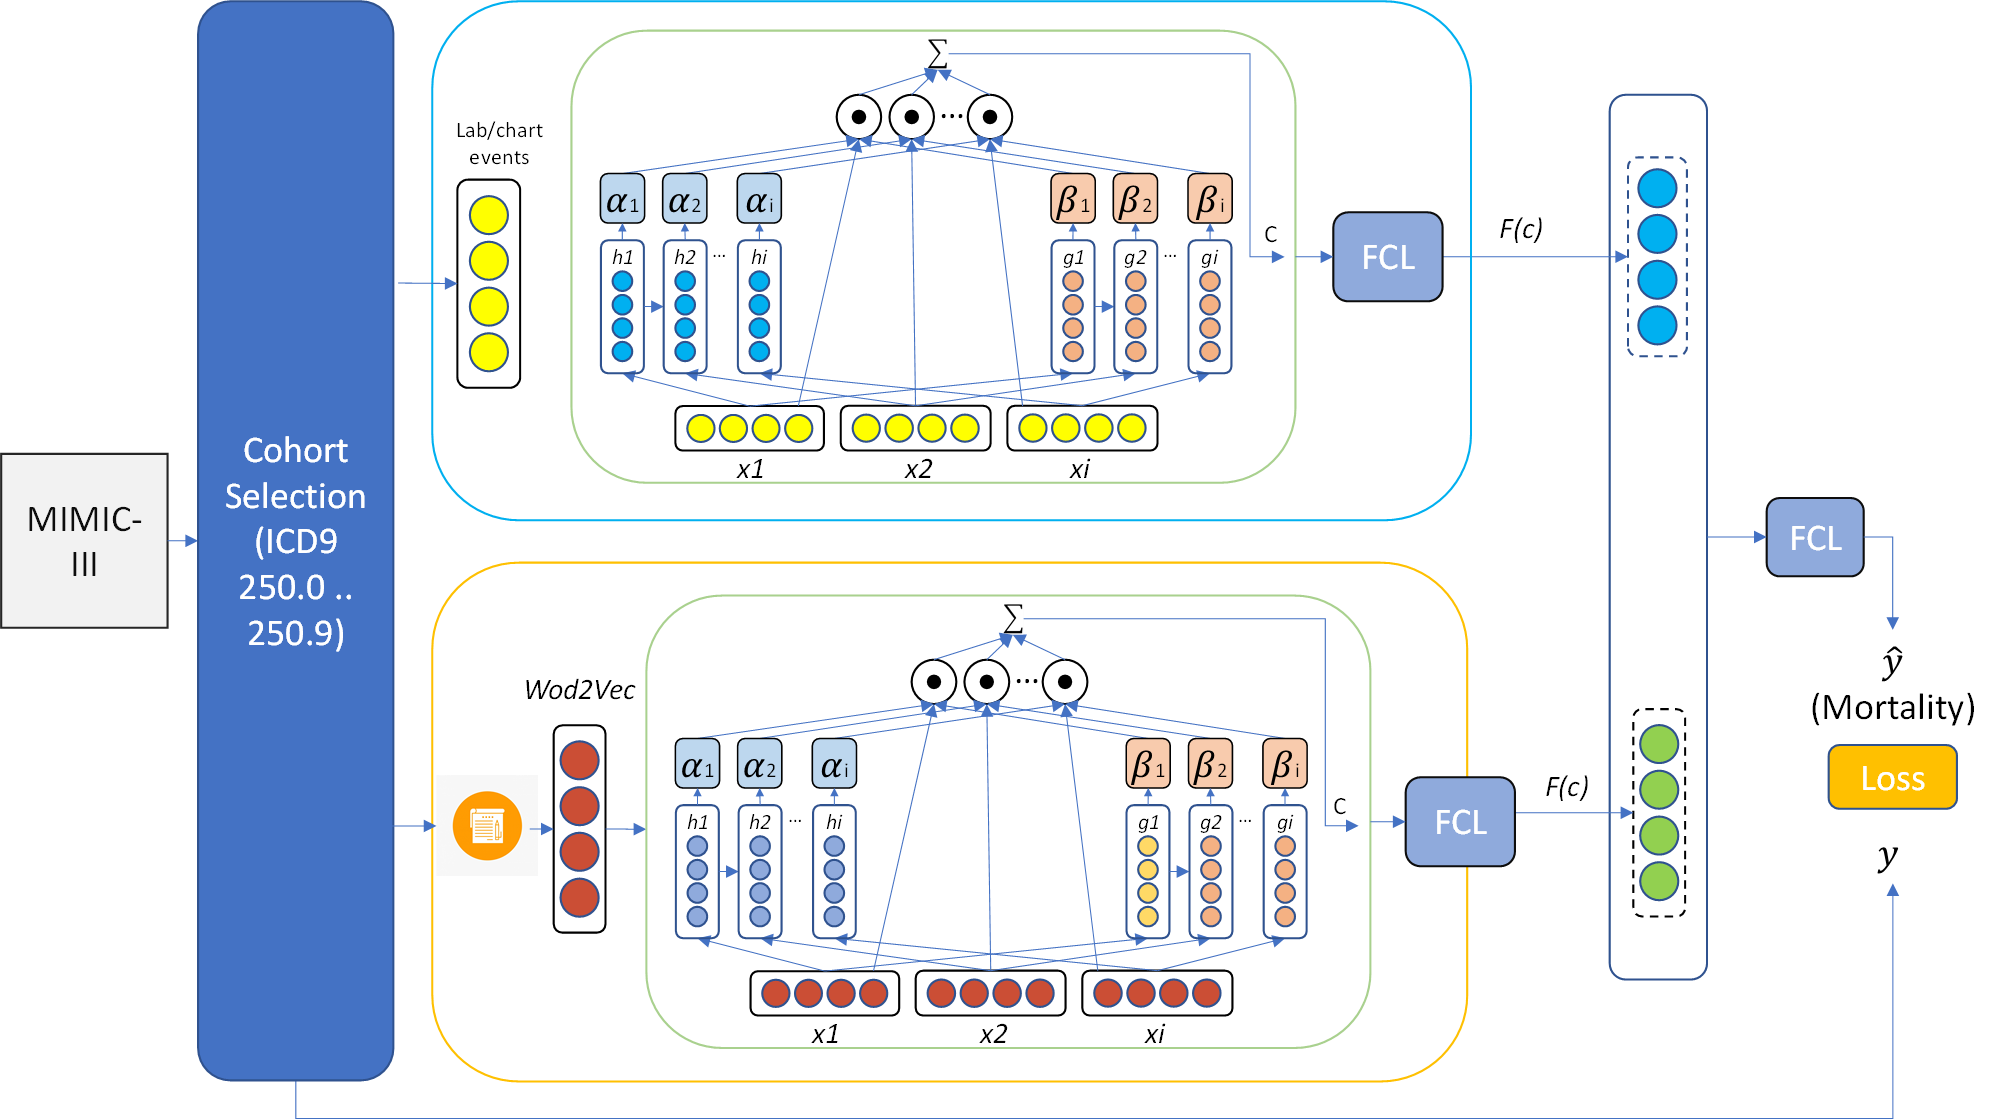
\includegraphics[width=2\columnwidth]{Model.png}
\caption{Model architecture.}
\label{fig:model}
\end{figure*}

Figure \ref{fig:model} depicts the network architecture of our model.

\subsection{Notes Network}

The Notes Network architecture consists of taking the clinical notes embedding 
described on the previous section and then feed it into two parallel RNN (GRUs) 
layers, to calculate on each its attention.  On one of them we calculate the 
attention for each distinct date ($\alpha$), and on the second one, we calculate the attention 
of each embedding component ($\beta$), followed by a FCL layer, and a sigmoid activation function, 
to output the embedding vectors for this network.

\subsection{Events Network}
The multi-hot vectors $\mathit v_i^{(p)}$  were used as inputs for the Events Network.  The architecture 
of this network comprises another pair of parallel RNNs (GRUs) with alpha ($\alpha$) and beta ($\beta$) attention, 
where $\alpha$ means the attention for each distinct event date, and $\beta$ means the attention for the different features. 
The network finally has a FCL and a sigmoid activation function to produce the embeddings vector of the events of each patient.


\subsection{Notes-Events Network}
The final Model takes the output of the two previous Networks (embedding vectors output of Notes and Events 
network were of size 128 each), concatenates them and applies two additional FCL layers with a dropout in the 
middle and a final sigmoid activation function to generate the final prediction.

\subsection{Normalization of attention weights}
Before extracting interpretable information from the attention weights of the events codes, the raw weights 
must be normalized to make them comparable with each other.  The normalization was done with the following 
transformation:

\begin{equation}
       \bar{\beta_i} = \frac{\sum_{b}\bar{e_i}^{(b)} \lvert\beta_i^{(b)}\rvert }{B}
\end{equation}

where $\beta_i$ is the normalized weight for event code $i$, $\bar{e_i}^{(b)}$ is the average of the values of event 
code $i$ in the batch $b$, $\bar{\beta_i}^{(b)}$ is the average of attention weights for event code $i$ 
in the batch $b$, and $B$ is the number of batches.  For this calculation the batch size was set to 1,000 patients.

\subsection{Experimental Setup}
The model was implemented in Pytorch 1.7.1 and trained initially in AWS Sagemaker environment 
with a memory of 8GBs. Eventually we moved the training to a more powerful machine with the same 
Pytorch version, but with 32GBs of RAM and an NVIDIA GeForce GTX 1060 with 6GB GPU. This enabled 
us to train the model and do fine tuning with much faster training times compared to only using 
the CPU environment.

\section{Experimental Results}
\subsection{Model assessment}
Table \ref{tab:assessment} shows the results of our model as we progressed in the construction and experimentation (always 10 epochs).

\begin{table*}
       \centering
       \caption{Model metrics.}
       \label{tab:assessment}
       \begin{tabular}{|c|c|c|c|c|c|c|c|c|c|} \hline
              \textbf{Notes Network}&	\textbf{Events Network	}&\textbf{Dataset}&	\textbf{Time}&	\textbf{LR}&	\textbf{Epochs}&	\textbf{Prec}&	\textbf{Recall}&	\textbf{F1}&	\textbf{ROC AUC} \\ \hline
       RNN	&RNN	&Unbalanced	&286.65	&0.001	&10	&0.6269	&0.367	&0.463	&0.871 \\ \hline
       RNN	&RNN	&Balanced	&566.94	&0.00001	&10	&0.1780	&0.948	&0.299	&0.765 \\ \hline
       RNN	&$\alpha$,$\beta$ Attn&	Unbalanced	&318.50	&0.001	&10	&0.6902	&0.516	&0.591	&0.879 \\ \hline
       RNN	&$\alpha$,$\beta$ Attn&	Balanced	&629.93	&0.00001	&10	&0.3912	&0.838	&0.533	&0.896 \\ \hline
       RNN	&$\alpha$,$\beta$ Attn&	Unbalanced	&279.23	&0.01	&10	&0.7280	&0.292	&0.417	 &0.845 \\ \hline
       RNN	&$\alpha$,$\beta$ Attn&	Balanced	&610.52	&0.0001	&10	&0.8470	&0.876	&0.861	 &0.974 \\ \hline
       $\alpha$ Attn&$\alpha$,$\beta$ Attn&	Unbalanced	&400.16	&0.001	&10	&0.7380	&0.397	&0.516	&0.879 \\ \hline
       $\alpha$ Attn&$\alpha$,$\beta$ Attn&	Balanced	&741.47	&0.0001	&10	&0.8770	&0.884	&0.880	&0.976 \\ \hline
       $\alpha$,$\beta$ Attn& $\alpha$,$\beta$ Attn& Unbalanced	&431.99	&0.001	&10	&0.6608	&0.521	&0.582	&0.908 \\ \hline
       $\alpha$,$\beta$ Attn& $\alpha$,$\beta$ Attn& Unbalanced	&434.23	&0.0001	&10	&0.6114	&0.493	&0.546	&0.893 \\ \hline
       $\alpha$,$\beta$ Attn& $\alpha$,$\beta$ Attn& Balanced	&852.77 &0.0001	&10 &0.8790	&0.868	&0.873	&0.977 \\ \hline
       
       \end{tabular}
\end{table*}

\subsection{Ranking of risk factors}
One of the advantages of attention mechanisms is the ability to produce interpretable models.  
In our case, we can take advantage of the attention weights to identify which of the clinical and 
paraclinical observations from chart and lab events has a bigger impact on the outcome of the patient.

Figure \ref{fig:att-weights} shows the normalized $\beta$ attention weights for each of the features considered 
in our model (features with less than 1,000 observations were left out of this analysis).

\graphicspath{ {figures/} } 
\begin{figure}[h]\centering
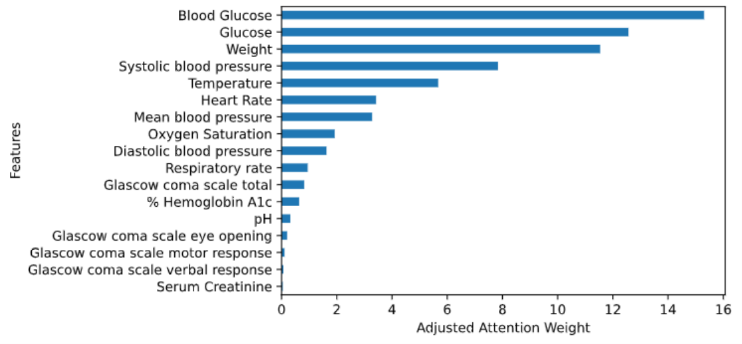
\includegraphics[width=1\columnwidth]{attention-weights.png}
\caption{Ranking of features according to the adjusted attention weights.}
\label{fig:att-weights}
\end{figure}

This is in line with the accepted view that high plasma glucose levels, 
high body mass index (BMI) and high blood pressure are risk factors commonly 
found together (\cite{lim}). 

To confirm that the most relevant features carry the information with most 
predictive power, we trained the model with just the eight features that received 
the most attention: blood glucose (lab event), glucose (chart event), weight, systolic 
blood pressure, temperature, heart rate, mean blood pressure, and oxygen saturation.  
After evaluation, these “essential” features’ model gave a precision of 0.622, recall of 0.390, 
f1 score of 0.873 and ROC AUC of 0.867.  The most dramatic difference between the full and the 
essential features model was on the recall (0.390 vs. 0.521) 21\% lower while the separation 
power (AUC ROC) was only 3\% lower (0.867 vs. 0.893) confirming that most of the information 
relevant for model performance was retained in the smaller features subset. 

\subsection{Contribution of each network module to the predictive power of the model.}
Next, we wanted to determine how much of the performance of the model comes from 
the clinical notes and how much comes from the sequences of chart and lab events.  

To determine this, we trained each network by itself and evaluated 
against our test sets, the results of the evaluations are shown in Table \ref{tab:networks-contributions}.

\begin{table*}
       \centering
       \caption{Contributions of each network module on model metrics.}
       \label{tab:networks-contributions}
       \begin{tabular}{|c|c|c|c|c|c|c|} \hline
              \textbf{Notes Network}&	\textbf{Events Network	}&\textbf{Dataset}&	\textbf{Prec}&	\textbf{Recall}&	\textbf{F1}&	\textbf{ROC AUC} \\ \hline      
              ---	&$\alpha$,$\beta$ Attn	&Unbalanced		&0.6033	&0.4644	&0.525	&0.850609 \\ \hline
              $\alpha$,$\beta$ Attn	&---	&Unbalanced		&0.625	&0.0199	&0.039	&0.78265 \\ \hline
              ---	&$\alpha$,$\beta$ Attn	&Balanced		&0.7319	&0.8632	&0.792	&0.960047 \\ \hline
              $\alpha$,$\beta$ Attn	&---	&Balanced		&0.7026	&0.8077	&0.751	&0.937759 \\ \hline
       \end{tabular}
\end{table*}

These results show that the clinical notes’ main contribution is on 
improving the general performance of the full model, but with a bigger 
improvement on the recall of the model or reducing the number of false 
negatives.  On the other hand, the main contribution of the lab and charts 
events is of course improving the overall performance; however, it is the 
precision that seems to be the one that increases the most, or, namely, 
reducing the number of false positives.   

Overall, the ability of the model to distinguish between classes, 
measured by AUC ROC, was reduced by 1.7\% when the clinical notes were 
ignored, and by 4\% when the lab and chart features were ignored.

\section{Discussion}
We analyzed the clinical notes of diabetic patients including the 
lab and other clinical features collected from the MIMICIII database 
and fed the data into parallel RNNs to predict mortality. We had 
originally attempted to use CNN on top of the Clinical Notes data, 
but after testing this, we switched to an RNN model as this makes easier 
the processing of the notes, and leads to a much faster training time. 

Our full network yielded good results compared to previous works, 
achieving a maximum AUC ROC of 0.977. We originally had observed a 
trade-off between the reported recall and precision when using the 
original training set, versus when using a balanced training set, 
but once we updated our models to include $\alpha$ and $\beta$ attention on both 
the Events and Notes network, the balanced cohort clearly yielded 
much better results, validating the idea of using a re-sampling 
algorithm to avoid our model from giving more weight to the majority class.

By ablating either one of the parallel RNN networks we were able to 
quantify the contribution that each module had in the outcome. With 
this approach we were able to determine that the events module 
captured most of the predictive power of the model (Table \ref{tab:networks-contributions}).  However, 
the notes module helped in improving its precision or reducing the number 
of false positives.  The clinical notes capture the medical insight 
that is not reflected in the objective chart and lab data.  One can 
speculate that this insight discriminates those patients that have 
good chances of surviving despite their poor looking chart and lab events.

The addition of attention mechanisms analogous to \textsc{RETAIN} 
(\cite{choi}) produced a significant improvement over the na\"ive 
RNNs (Table \ref{tab:assessment}).  The ROC AUC improved from 0.765 to 0.896 after 
the addition of the two-level attention mechanism in the events 
module, and to 0.977 after implementing attention also in the notes’ 
module. The magnitude of these improvements was striking, being much 
higher than those reported in the original publication (\cite{choi}).  
Although, attention mechanisms have shown similar degrees of improvement 
on text classification applications (\cite{minaee}).

Using this attention-based model we were able to identify those 
features from the APACHE II score that are more relevant for predicting 
the outcome of the patient (Figure 3).  Retraining the model with 
just eight of these features was able to produce an ROC AUC just 11\% 
lower than the one obtained with the full feature set.  The essential 
features set comprised vital signs and measurements such as blood glucose, 
weight, blood pressure, temperature, heart rate, and oxygen saturation.  
The association of some of these entities with a poor health in diabetes 
patients is well documented in the clinical literature (Church et al., 2004).  
The fact that our deep learning model was able to draw conclusions like large 
population studies is remarkable.  The power of deep learning algorithms 
to extract valuable clinical information that is hidden in EHR data cannot 
be overstated.  These insights raise the question on the application of 
APACHE II score to rank diabetic patients in ICU.  Getting correct APACHE II 
scores require adherence to strict guidelines and regular training of 
medical staff (\cite{polderman}).  A reduction on the number 
of dimensions that need to be considered to calculate the score without 
losing its predictive capability could be seen as an improvement in diabetic 
patient care.

\section{Conclusion/Optimization}
We developed a multi-network multi-attention deep learning model 
to predict the mortality of diabetic ICU patients 48 hrs before 
discharge. The evaluation of the model reported an AUC ROC that is 
higher than previous similar models. The model is a step further of 
previous works by engaging multiple networks and using both clinical 
notes and clinical features as source to parallel RNNs as well as 
implementing multi-attention on each of the parallel networks in the 
prediction task. This model is an improvement in the right direction, 
which could be integrated in the clinical setting to manage the 
extensive resources that are being expended on diabetic patients 
and increase the efficiency of clinicians in the ICU.

Further optimization can be explored in the future to improve the 
scores and validate the results found in other datasets of similar 
composition. Additionally, further work is required to ensure the 
resiliency of the model by implementing k-fold cross validation with 
resampling as well as testing the trained model against inputs that 
have noise, that is, inputs that have certain random additional components.  
Another area of exploration is to analyze whether making additional 
pre-processing of the lab/chart events features, like normalization 
of the values would improve the performance or resiliency of the model. 
In addition, the continuous numerical values from the chart and lab 
events can be converted to categorical values (e.g. below normal range, 
normal range, above normal range).  Categorical input values could be 
represented in one-hot encodings and it might be easier for the model to 
learn their patterns of distribution.  

An interesting perspective that might be worth furthering the project on, 
would be to consider different observation window for the note, instead of 
the 48 hrs we used for the project, a window of 24 hrs or lesser time 
frame could be considered.

\section{Team Contributions}
\begin{itemize}
       \item Olabisi Balogun
       \begin{itemize}
              \item Worked on creating the different tables required for training the models.
              \item Created the \textsc{sql\_queries} file
              \item Trained the Word Embedding Model
              \item Worked on the project report
              \item Worked on the project slides
              \item Documented the Readme file
       \end{itemize}
       \item Jorge Flores
       \begin{itemize}
              \item Redesigned the main cohort table
              \item Created the \textsc{notes\_extraction} code
              \item Trained the note network model
              \item Worked on the joint model
              \item Performed ablation experiment.
              \item Worked on the project report
              \item Worked on the project slides
       \end{itemize}
       \item Francisco Noya
       \begin{itemize}
              \item Created the \textsc{events\_extraction} code
              \item Trained the events network model.
              \item Worked on the joint model
              \item Performed risk factors experiment.
              \item Performed ablation experiment.
              \item Worked on the project report
              \item Worked on the project slides
       \end{itemize}
\end{itemize}

\section{Code Repository}
\begin{itemize}
       \item \href{https://github.com/fnoya/dlh-project}{Github}
       \item \href{https://drive.google.com/drive/folders/1KMSbvsonOh3s8L902e-ExIgh_IgH0VnV?usp=sharing}{Google Drive}: data processing files included, *.p, *.npy.
\end{itemize}

\section {Presentation Video}
\begin{itemize}
       \item \url{https://youtu.be/FaJ5Of8TVMs }
\end{itemize}

\begin{thebibliography}{6}
       \bibitem{anand}
       Anand, R. S., Stey, P., Jain, S., Biron, D. R., Bhatt, H., Monteiro, K., Feller, E., Ranney, M. L., Sarkar, I. N., \& Chen, E. S. (2018). ``Predicting mortality in diabetic ICU patients using machine learning and severity indices''. \textit{AMIA Summits on Translational Science Proceedings}, 2018, 310.
       \bibitem{che}
       Che, Z., Purushotham, S., Cho, K., Sontag, D., \& Liu, Y. (2018). ``Recurrent neural networks for multivariate time series with missing values''. \textit{Scientific reports}, 8(1), 1-12.
       \bibitem{choi}
       Choi, E., Mohammad, Joshua, Schuetz, A., Walter, \& Sun, J. (2017). ``RETAIN: An Interpretable Predictive Model for Healthcare using Reverse Time Attention Mechanism''. \textit{arXiv pre-print arxiv:1608.05745}.
       \bibitem{church}
       Church, T. S., Cheng, Y. J., Earnest, C. P., Barlow, C. E., Gibbons, L. W., Priest, E. L., \& Blair, S. N. (2004). Exercise Capacity and Body Composition as Predictors of Mortality Among Men With Diabetes. \textit{Diabetes Care}, 27(1), 83-88. \url{https://doi.org/10.2337/diacare.27.1.83}.
       \bibitem{egan}
       Egan, A. M., \& Dinneen, S. F. (2019). ``What is diabetes?''. \textit{Medicine}, 47(1), 1-4.
       \bibitem{gregg}
       Gregg, E. W., Cheng, Y. J., Srinivasan, M., Lin, J., Geiss, L. S., Albright, A. L., \& Imperatore, G. (2018). ``Trends in cause-specific mortality among adults with and without diagnosed diabetes in the USA: an epidemiological analysis of linked national survey and vital statistics data''. \textit{The Lancet}, 391(10138), 2430-2440.
       \bibitem{johnson}
       Johnson, Alistair, et al. ``MIMIC-III Clinical Database (version 1.4).'', \textit{Physionet}, September 2016, \url{https://doi.org/10.13026/C2XW26}
       \bibitem{knaus}
       Knaus, W. A., Draper, E. A., Wagner, D. P., \& Zimmerman, J. E. (1985). ``APACHE II: a severity of disease classification system''. \textit{Critical care medicine}, 13(10), 818-829.
       \bibitem{kumar}
       Kumar, B. (2020). ``10 Techniques to deal with Imbalanced Classes in Machine Learning''. Analytics Vidhya. \href{https://www.analyticsvidhya.com/blog/2020/07/10-techniques-to-deal-with-class-imbalance-in-machine-learning/}{https://www.analyticsvidhya.com/blog/2020/07/}.
       \bibitem{lim}
       Lim, Vos, Flaxman, Danaei et al. (2012). ``A comparative risk assessment of burden of disease and injury attributable to 67 risk factors and risk factor clusters in 21 regions, 1990–2010: a systematic analysis for the Global Burden of Disease Study 2010''.  \textit{The Lancet}, 380(9859), 2224-2260.       \bibitem{minaee}
       Minaee, S., Kalchbrenner, N., Cambria, E., Nikzad, N., Chenaghlu, M., \& Gao, J. (2021). Deep Learning--based Text Classification: A Comprehensive Review. \textit{ACM Comput. Surv.}, 54(3), Article 62. \url{https://doi.org/10.1145/3439726}
       \bibitem{polderman}
       Polderman, K. H., Girbes, A. R. J., Thijs, L. G., \& Strack Van Schijndel, R. J. M.. (2001). Accuracy and reliability of APACHE II scoring in two intensive care units. \textit{Anaesthesia}, 56(1), 47–50. \url{https://doi.org/10.1046/j.1365-2044.2001.01763.x}
       \bibitem{yang}
       Yang, H., Kuang, L., \& Xia, F. (2021). ``Multimodal temporal-clinical note network for mortality prediction''. \textit{Journal of Biomedical Semantics}, 12(1), 1-14.
       \bibitem{ye}
       Ye, J., Yao, L., Shen, J., Janarthanam, R., \& Luo, Y. (2020). ``Predicting mortality in critically ill patients with diabetes using machine learning and clinical notes''. \textit{BMC Medical Informatics and Decision Making}, 20(11), 1-7.
       \bibitem{zimmet}
       Zimmet, P. Z., Magliano, D. J., Herman, W. H., \& Shaw, J. E. (2014). ``Diabetes: a 21st century challenge''. \textit{The Lancet Diabetes \& endocrinology}, 2(1), 56-64.

\end{thebibliography}
              
\end{document}
